\section{Experiments}
\label{sec:experiments}

In this section, we conduct extensive evaluations in both simulation and
real-world environments to assess \method and its memory-augmented extension,
\memmethod.
Specifically, our experiments are designed to answer the following research
questions:
\begin{itemize}
    \item[Q1:] How effectively do \method and \memmethod learn 3D manipulation
    compared with state-of-the-art methods when sufficient demonstrations are
    available?

    \item[Q2:] How robust are \method and \memmethod under
    out-of-distribution conditions, including distractors, lighting changes,
    background variations, novel object--skill combinations, and unseen
    object categories?

    \item[Q3:] How important are the proposed architectural components,
    including heatmap-based action decoding, 2D heatmap pre-training, and
    unified spatio-temporal memory, to the overall performance?

    \item[Q4:] Can \method and \memmethod be deployed effectively across
    different real-world robot platforms while retaining high sample
    efficiency, such as learning each task from only 10 demonstrations?

    \item[Q5:] How effectively can \memmethod address memory-dependent manipulation tasks?
\end{itemize}

\subsection{RLBench: General 3D Manipulation}
\label{sec:exp:bridgevla}
\label{sec:exp:rlbench}

To evaluate the base model's capacity for general 3D manipulation, we primarily evaluate \method\ and \memmethod\ on the RLBench benchmark.

\begin{table*}[!t]
\centering
\caption{\textbf{Results and ablation studies on RLBench.}
Success rates (SR, \%) across 18 tasks, together with the average SR and
average rank (lower is better).
The upper rows report prior methods, followed by \method
(the memory-free base policy, also referred to as \textbf{Base}) and
\memmethod; the indented rows below each report its architectural and
memory ablations.
Results are presented as mean$_{\pm\mathrm{std}}$ over five random seeds,
with 25 evaluation episodes per seed.
\textbf{w/o}~$\mathcal{S}$ and \textbf{w/o}~$\mathcal{T}$ denote
\memmethod without spatial and temporal memory, respectively.
Evaluation protocols and training details are provided in
Appendices~\ref{app:finetune_hparams} and~\ref{app:eval_protocol}.
The best result in each column is highlighted in bold.}
\label{tab:rlbench}
\scriptsize
\setlength{\tabcolsep}{3pt}
% zero rule separation; \arraystretch below compensates the row height
\setlength{\aboverulesep}{0pt}
\setlength{\belowrulesep}{0pt}
\renewcommand{\arraystretch}{1.15}
\resizebox{\fitwidth}{!}{%
\begin{tabular}{l *{10}{c}}
\toprule
& \textbf{Avg.} & \textbf{Avg.} & \textbf{Close} & \textbf{Drag} & \textbf{Insert}
& \textbf{Meat off} & \textbf{Open} & \textbf{Place} & \textbf{Place}
& \textbf{Push} \\
\multirow{-2}{*}{\textbf{Method}}
& \textbf{SR (\%) $\uparrow$} & \textbf{Rank $\downarrow$} & \textbf{Jar} & \textbf{Stick} & \textbf{Peg}
& \textbf{Grill} & \textbf{Drawer} & \textbf{Cups} & \textbf{Wine}
& \textbf{Buttons} \\
\midrule
PerAct~\cite{shridhar2023perceiver} & 49.4 & 11.33 & 55.2$_{\pm 4.7}$ & 89.6$_{\pm 4.1}$ & 5.6$_{\pm 4.1}$ & 70.4$_{\pm 2.0}$ & 88.0$_{\pm 5.7}$ & 2.4$_{\pm 3.2}$ & 44.8$_{\pm 7.8}$ & 92.8$_{\pm 3.0}$ \\
Act3D~\cite{gervet2023act3d} & 65.0 & 9.17 & 92.0 & 92.0 & 27.0 & 94.0 & 93.0 & 3.0 & 80.0 & 99.0 \\
RVT~\cite{goyal2023rvt} & 62.9 & 9.08 & 52.0$_{\pm 2.5}$ & 99.2$_{\pm 1.6}$ & 11.2$_{\pm 3.0}$ & 88.0$_{\pm 2.5}$ & 71.2$_{\pm 6.9}$ & 4.0$_{\pm 2.5}$ & 91.0$_{\pm 5.2}$ & \textbf{100.0}$_{\pm 0.0}$ \\
3D Diffuser Actor~\cite{3d-da} & 81.3 & 6.19 & 96.0$_{\pm 2.5}$ & \textbf{100.0}$_{\pm 0.0}$ & 65.6$_{\pm 4.1}$ & 96.8$_{\pm 1.6}$ & 89.6$_{\pm 4.1}$ & 24.0$_{\pm 7.6}$ & 93.6$_{\pm 4.8}$ & 98.4$_{\pm 2.0}$ \\
RVT-2~\cite{goyal2024rvt} & 81.4 & 5.97 & \textbf{100.0}$_{\pm 0.0}$ & 99.0$_{\pm 1.7}$ & 40.0$_{\pm 0.0}$ & 99.0$_{\pm 1.7}$ & 74.0$_{\pm 11.8}$ & 38.0$_{\pm 4.5}$ & 95.0$_{\pm 3.3}$ & \textbf{100.0}$_{\pm 0.0}$ \\
SAM2Act~\cite{fang2025sam2act} & 86.8$_{\pm 0.5}$ & 5.47 & 99.0$_{\pm 2.0}$ & 99.0$_{\pm 2.0}$ & 84.0$_{\pm 5.7}$ & 98.0$_{\pm 2.3}$ & 83.0$_{\pm 6.0}$ & 47.0$_{\pm 6.0}$ & 93.0$_{\pm 3.8}$ & \textbf{100.0}$_{\pm 0.0}$ \\
\midrule
\textbf{\method\ (ours)} & 90.5$_{\pm 1.1}$ & 4.75 & \textbf{100.0}$_{\pm 0.0}$ & 97.6$_{\pm 3.6}$ & 91.2$_{\pm 1.8}$ & \textbf{100.0}$_{\pm 0.0}$ & 99.2$_{\pm 1.8}$ & 58.4$_{\pm 4.6}$ & 89.6$_{\pm 8.3}$ & \textbf{100.0}$_{\pm 0.0}$ \\
\tbranch w/ discretized rotation & 88.2 & 4.86 & \textbf{100.0}$_{\pm 0.0}$ & \textbf{100.0}$_{\pm 0.0}$ & 88.0$_{\pm 2.8}$ & \textbf{100.0}$_{\pm 0.0}$ & \textbf{100.0}$_{\pm 0.0}$ & 58.4$_{\pm 10.0}$ & 88.0$_{\pm 2.8}$ & 98.4$_{\pm 2.2}$ \\
\tbranch w/o heatmap decoding & 31.4 & 12.78 & 49.3$_{\pm 2.3}$ & 65.3$_{\pm 2.3}$ & 0.0$_{\pm 0.0}$ & 81.3$_{\pm 4.6}$ & 74.7$_{\pm 10.1}$ & 1.3$_{\pm 2.3}$ & 32.0$_{\pm 14.4}$ & 54.7$_{\pm 6.1}$ \\
\tlast w/ 3D position input & 56.2 & 10.14 & 96.0$_{\pm 0.0}$ & 58.7$_{\pm 6.1}$ & 26.7$_{\pm 2.3}$ & 96.0$_{\pm 0.0}$ & 97.3$_{\pm 2.3}$ & 14.7$_{\pm 4.6}$ & 81.3$_{\pm 8.3}$ & 86.7$_{\pm 2.3}$ \\
\specialrule{1pt}{0pt}{0pt}
\textbf{\memmethod\ (ours)} & \textbf{93.7$_{\pm 0.6}$} & \textbf{3.64} & \textbf{100.0}$_{\pm 0.0}$ & 98.4$_{\pm 2.2}$ & \textbf{99.2}$_{\pm 1.8}$ & \textbf{100.0}$_{\pm 0.0}$ & 99.2$_{\pm 1.8}$ & \textbf{76.8}$_{\pm 11.5}$ & \textbf{95.2}$_{\pm 4.4}$ & \textbf{100.0}$_{\pm 0.0}$ \\
\tbranch w/o spatial memory & 92.0$_{\pm 0.5}$ & 3.81 & \textbf{100.0}$_{\pm 0.0}$ & \textbf{100.0}$_{\pm 0.0}$ & 95.2$_{\pm 3.3}$ & \textbf{100.0}$_{\pm 0.0}$ & 99.2$_{\pm 1.8}$ & 74.4$_{\pm 3.6}$ & 78.4$_{\pm 3.6}$ & \textbf{100.0}$_{\pm 0.0}$ \\
\tlast w/o temporal memory & 91.9$_{\pm 1.0}$ & 3.81 & \textbf{100.0}$_{\pm 0.0}$ & 99.2$_{\pm 1.8}$ & 82.4$_{\pm 2.2}$ & \textbf{100.0}$_{\pm 0.0}$ & 97.6$_{\pm 2.2}$ & 57.6$_{\pm 7.3}$ & 90.4$_{\pm 4.6}$ & \textbf{100.0}$_{\pm 0.0}$ \\
\bottomrule
\addlinespace[5pt]
\toprule
& \textbf{Put in} & \textbf{Put in} & \textbf{Put in} & \textbf{Screw}
& \textbf{Slide} & \textbf{Sort} & \textbf{Stack} & \textbf{Stack}
& \textbf{Sweep to} & \textbf{Turn} \\
\multirow{-2}{*}{\textbf{Method}}
& \textbf{Cupboard} & \textbf{Drawer} & \textbf{Safe} & \textbf{Bulb}
& \textbf{Block} & \textbf{Shape} & \textbf{Blocks} & \textbf{Cups}
& \textbf{Dustpan} & \textbf{Tap} \\
\midrule
PerAct~\cite{shridhar2023perceiver} & 28.0$_{\pm 4.4}$ & 51.2$_{\pm 4.7}$ & 84.0$_{\pm 3.6}$ & 17.6$_{\pm 2.0}$ & 74.0$_{\pm 13.0}$ & 16.8$_{\pm 4.7}$ & 26.4$_{\pm 3.2}$ & 2.4$_{\pm 2.0}$ & 52.0$_{\pm 0.0}$ & 88.0$_{\pm 4.4}$ \\
Act3D~\cite{gervet2023act3d} & 51.0 & 90.0 & 95.0 & 47.0 & 93.0 & 8.0 & 12.0 & 9.0 & 92.0 & 94.0 \\
RVT~\cite{goyal2023rvt} & 49.6$_{\pm 3.2}$ & 88.0$_{\pm 5.7}$ & 91.2$_{\pm 3.0}$ & 48.0$_{\pm 5.7}$ & 81.6$_{\pm 5.4}$ & 36.0$_{\pm 2.5}$ & 28.8$_{\pm 3.9}$ & 26.4$_{\pm 8.2}$ & 72.0$_{\pm 0.0}$ & 93.6$_{\pm 4.1}$ \\
3D Diffuser Actor~\cite{3d-da} & 85.6$_{\pm 4.1}$ & 96.0$_{\pm 3.6}$ & 97.6$_{\pm 2.0}$ & 82.4$_{\pm 2.0}$ & 97.6$_{\pm 3.2}$ & 44.0$_{\pm 4.4}$ & 68.3$_{\pm 3.3}$ & 47.2$_{\pm 8.5}$ & 84.0$_{\pm 4.4}$ & \textbf{99.2}$_{\pm 1.6}$ \\
RVT-2~\cite{goyal2024rvt} & 66.0$_{\pm 4.5}$ & 96.0$_{\pm 0.0}$ & 96.0$_{\pm 2.8}$ & 88.0$_{\pm 4.9}$ & 92.0$_{\pm 2.8}$ & 35.0$_{\pm 7.1}$ & 80.0$_{\pm 2.8}$ & 69.0$_{\pm 5.9}$ & \textbf{100.0}$_{\pm 0.0}$ & 99.0$_{\pm 1.7}$ \\
SAM2Act~\cite{fang2025sam2act} & 75.0$_{\pm 3.8}$ & 99.0$_{\pm 2.0}$ & 98.0$_{\pm 2.3}$ & 89.0$_{\pm 2.0}$ & 86.0$_{\pm 4.0}$ & 64.0$_{\pm 4.6}$ & 76.0$_{\pm 8.6}$ & 78.0$_{\pm 4.0}$ & 99.0$_{\pm 2.0}$ & 96.0$_{\pm 5.7}$ \\
\midrule
\textbf{\method\ (ours)} & 91.2$_{\pm 1.8}$ & 96.0$_{\pm 0.0}$ & 95.2$_{\pm 3.3}$ & 93.6$_{\pm 6.1}$ & 95.2$_{\pm 3.3}$ & 55.2$_{\pm 5.2}$ & 84.8$_{\pm 9.1}$ & 88.8$_{\pm 3.3}$ & \textbf{100.0}$_{\pm 0.0}$ & 92.8$_{\pm 3.3}$ \\
\tbranch w/ discretized rotation & 73.6$_{\pm 4.6}$ & \textbf{99.2}$_{\pm 1.8}$ & \textbf{99.2}$_{\pm 1.8}$ & 87.2$_{\pm 6.6}$ & 96.0$_{\pm 2.8}$ & 60.8$_{\pm 7.7}$ & 76.8$_{\pm 8.7}$ & 81.6$_{\pm 3.6}$ & 87.2$_{\pm 1.8}$ & 92.8$_{\pm 3.3}$ \\
\tbranch w/o heatmap decoding & 5.3$_{\pm 2.3}$ & 0.0$_{\pm 0.0}$ & 58.7$_{\pm 22.7}$ & 2.7$_{\pm 2.3}$ & 64.0$_{\pm 0.0}$ & 4.0$_{\pm 4.0}$ & 0.0$_{\pm 0.0}$ & 0.0$_{\pm 0.0}$ & 32.0$_{\pm 4.0}$ & 40.0$_{\pm 10.6}$ \\
\tlast w/ 3D position input & 10.7$_{\pm 2.3}$ & 78.7$_{\pm 2.3}$ & 97.3$_{\pm 4.6}$ & 16.0$_{\pm 4.0}$ & 72.0$_{\pm 0.0}$ & 21.3$_{\pm 8.3}$ & 17.3$_{\pm 2.3}$ & 4.0$_{\pm 4.0}$ & 53.3$_{\pm 2.3}$ & 84.0$_{\pm 0.0}$ \\
\specialrule{1pt}{0pt}{0pt}
\textbf{\memmethod\ (ours)} & \textbf{92.0}$_{\pm 0.0}$ & \textbf{99.2}$_{\pm 1.8}$ & 92.8$_{\pm 5.9}$ & 95.2$_{\pm 5.2}$ & 96.0$_{\pm 4.0}$ & 72.0$_{\pm 6.3}$ & 85.6$_{\pm 4.6}$ & \textbf{98.4}$_{\pm 2.2}$ & 97.6$_{\pm 2.2}$ & 89.6$_{\pm 4.6}$ \\
\tbranch w/o spatial memory & 90.4$_{\pm 2.2}$ & 91.2$_{\pm 1.8}$ & 96.0$_{\pm 4.9}$ & 95.2$_{\pm 1.8}$ & 97.6$_{\pm 3.6}$ & 60.8$_{\pm 3.3}$ & \textbf{91.2}$_{\pm 3.3}$ & 92.8$_{\pm 4.4}$ & 99.2$_{\pm 1.8}$ & 95.2$_{\pm 4.4}$ \\
\tlast w/o temporal memory & 88.8$_{\pm 4.4}$ & 98.4$_{\pm 3.6}$ & 92.8$_{\pm 3.3}$ & \textbf{96.0}$_{\pm 4.0}$ & \textbf{100.0}$_{\pm 0.0}$ & \textbf{73.6}$_{\pm 5.4}$ & 88.8$_{\pm 3.3}$ & 93.6$_{\pm 2.2}$ & \textbf{100.0}$_{\pm 0.0}$ & 94.4$_{\pm 4.6}$ \\
\bottomrule
\end{tabular}%
}
\end{table*}


\paragraph{Setup} 
RLBench~\cite{james2020rlbench} serves as a standard multi-task suite for evaluating manipulation policies.
It implements tasks in CoppeliaSim~\cite{rohmer2013v} using a Franka Panda robot equipped with a parallel-jaw gripper, with observations provided by four RGB-D cameras (front, left shoulder, right shoulder, and wrist). 
Following previous works~\cite{shridhar2023perceiver,goyal2023rvt,goyal2024rvt}, we evaluate on 18 tasks spanning non-prehensile manipulation such as \textit{Slide Block to Target}, pick-and-place tasks like \textit{Stack Cups}, and high-precision insertion tasks including \textit{Sort Shape}. 
We train on 100 demonstrations per task and report the mean success rate over five evaluation runs of 25 episodes per task.

\paragraph{Baselines}
We compare \method\ with state-of-the-art baselines encompassing both 2D and 3D methods.
(1) \textbf{PerAct}~\cite{shridhar2023perceiver} operates in the voxel space and predicts the action with a Perceiver transformer~\cite{jaegleperceiver}.
(2) \textbf{Act3D}~\cite{gervet2023act3d} predicts the next keyframe action by selecting the point with the highest score from a set of randomly sampled points in the workspace.
(3) \textbf{RVT}~\cite{goyal2023rvt} uses a multi-view transformer to aggregate information from multiple orthographic views of the point cloud observation.
(4) \textbf{3D Diffuser Actor}~\cite{3d-da} generates 3D trajectories via a diffusion process conditioned on the 3D observation and language instruction.
(5) \textbf{RVT-2}~\cite{goyal2024rvt} further improves the precision of its prior via a coarse-to-fine strategy.
(6) \textbf{SAM2Act}~\cite{fang2025sam2act}, the previous state-of-the-art method on this benchmark, builds upon the multi-view transformer and integrates the SAM2 visual foundation model to strengthen scene representation.

\paragraph{Results} 
Table~\ref{tab:rlbench} summarizes the performance comparison. \method\ achieves a 90.5\% average success rate across the 18 tasks, outperforming SAM2Act by 3.7 absolute percentage points, establishing a new state-of-the-art and addressing Q1.
This improvement is particularly pronounced in precision-critical tasks such as \emph{Stack Cups}, underscoring the efficacy of our dense per-view heatmap representation for fine-grained localization. The high success rates showcase its strong capability in precise manipulation. 
The primary failure modes emerge in occlusion-heavy tasks, where the robot's arm obscures the target during the fine-localization stage.
These occlusions are later resolved by \memmethod's spatio-temporal memory, which elevates the overall success rate to 93.7\% and brings significant gains to \emph{Sort Shape} (+16.8\%) and \emph{Place Cups} (+18.4\%).
The indented rows of Table~\ref{tab:rlbench} report ablated variants of both models, which we analyze in Sec.~\ref{sec:exp:ablation}.
% RMBench (the main memory experiment) is declared first so it takes the lower
% table number and both full-width tables float together onto a page before the
% real-robot setup figure; its discussion follows in Sec.~\ref{sec:exp:rmbench}.
\begin{table*}[!t]
\centering
\caption{\textbf{Results on RMBench.}
Success rates (\%) over 100 episodes per task on the nine dual-arm
RMBench tasks~\cite{chen2026rmbench}, grouped by task memory
complexity.
Baseline numbers are quoted
from~\cite{chen2026rmbench,yang2026memorywam,yang2026wla}, with group
averages recomputed from per-task results where a source reports none.
Best result per task in bold; ``--'' denotes tasks not evaluated by the
source.}
\label{tab:rmbench_main}
\footnotesize
\setlength{\tabcolsep}{4pt}
% zero rule separation; \arraystretch below compensates the row height
\setlength{\aboverulesep}{0pt}
\setlength{\belowrulesep}{0pt}
\renewcommand{\arraystretch}{1.25}
\begin{tabular}{l c cccccc ccccc}
\toprule
& & \multicolumn{6}{c}{\textbf{$M(1)$ tasks}}
& \multicolumn{5}{c}{\textbf{$M(n)$ tasks}} \\
\cmidrule(lr){3-8} \cmidrule(lr){9-13}
& \textbf{Overall}
& \textbf{Observe \&} & \textbf{Rearrange} & \textbf{Put Back} & \textbf{Swap} & \textbf{Swap} &
& \textbf{Battery} & \textbf{Blocks} & \textbf{Cover} & \textbf{Press} & \\
\multirow{-2}{*}{\textbf{Method}}
& \textbf{Avg.}
& \textbf{Pick Up} & \textbf{Blocks} & \textbf{Block} & \textbf{Blocks} & \textbf{T} & \multirow{-2}{*}{\textbf{\textit{Avg.}}}
& \textbf{Try} & \textbf{Ranking Try} & \textbf{Blocks} & \textbf{Button} & \multirow{-2}{*}{\textbf{\textit{Avg.}}} \\
\midrule
DP~\cite{chi2024diffusionpolicy}        & 5.8  & 1  & 0   & 0   & 11  & 20 & 6.4  & 10 & 10  & 0  & 0  & 5.0  \\
ACT~\cite{zhao2023learning}             & 5.9  & 1  & 29  & 0   & 2   & 2  & 6.8  & 19 & 0   & 0  & 0  & 4.8  \\
$\pi_{0.5}$~\cite{intelligence2025pi_}  & 10.4 & 9  & 13  & 11  & 24  & 15 & 14.4 & 16 & 6   & 0  & 0  & 5.5  \\
X-VLA~\cite{zheng2025xvla}              & 9.8  & 9  & 13  & 18  & 16  & 3  & 11.8 & 26 & 1   & 2  & 0  & 7.3  \\
Mem-0~\cite{chen2026rmbench}            & 42.0 & 4  & 89  & 90  & 67  & 14 & 52.8 & 28 & 18  & 68 & 0  & 28.5 \\
Fast-WAM~\cite{yuan2026fastwam}         & 5.9  & 0  & 0   & 0   & 0   & 7  & 1.4  & 20 & 26  & 0  & 0  & 11.5 \\
LingBot-VA~\cite{li2026lingbotva}       & 78.2 & 13 & \textbf{100} & \textbf{100} & 99  & 88 & 80.0 & 41 & \textbf{100} & 79 & 84 & 76.0 \\
MemoryWAM~\cite{yang2026memorywam}      & 83.0 & 27 & \textbf{100} & \textbf{100} & \textbf{100} & 94 & 84.2 & 41 & \textbf{100} & 98 & 87 & 81.5 \\
\midrule
\textbf{\method\ (ours)}                & 18.9 & 75 & 0   & 1   & 11 & 8  & 19.0 & 72 & 0   & 3  & 0  & 18.8 \\
\textbf{\memmethod\ (ours)}             & \textbf{96.0} & \textbf{81} & \textbf{100} & \textbf{100} & 99 & \textbf{96} & \textbf{95.2} & \textbf{96} & \textbf{100} & \textbf{99} & \textbf{93} & \textbf{97.0} \\
\bottomrule
\end{tabular}
\end{table*}

\begin{table*}[!t]
\centering
\caption{\textbf{Results on COLOSSEUM.}
Success rates (\%) across the 14 COLOSSEUM evaluation
settings~\cite{pumacay2024colosseum}: the 12 individual perturbation
axes, the original RLBench variations (``RLBench''), and all
perturbations applied jointly (``All Perturb.'').
MO and RO denote perturbations of the manipulated object and the
receptacle object, respectively.
``Avg.\ Rank'' is the average rank across the 14 settings over all
listed methods (lower is better).
R3M-MLP, MVP-MLP, PerAct, and RVT are quoted
from~\cite{pumacay2024colosseum}; RVT-2, \method, and \memmethod\ were
trained and evaluated by us (mean$\pm$variance over three test
repetitions; Appendix~\ref{app:eval_protocol}).
Best result per column in bold.}
\label{tab:colosseum}
\footnotesize
\setlength{\tabcolsep}{4pt}
% zero rule separation; \arraystretch below compensates the row height
\setlength{\aboverulesep}{0pt}
\setlength{\belowrulesep}{0pt}
\renewcommand{\arraystretch}{1.25}
\resizebox{\fitwidth}{!}{%
\begin{tabular}{l*{8}{c}}
\toprule
& \textbf{Avg.} & \textbf{Avg.} & \textbf{All} & \textbf{MO} & \textbf{RO} & \textbf{MO} & \textbf{RO} & \textbf{MO} \\
\multirow{-2}{*}{\textbf{Method}}
& \textbf{SR (\%) $\uparrow$} & \textbf{Rank $\downarrow$} & \textbf{Perturb.} & \textbf{Color} & \textbf{Color} & \textbf{Texture} & \textbf{Texture} & \textbf{Size} \\
\midrule
R3M-MLP~\cite{nair2022r3m}          & 0.8  & 6.71 & 0.6  & 0.4  & 0.0  & 0.0  & 0.0   & 1.8 \\
% NOTE: MVP-MLP Avg 1.6 reproduced as published; recomputation from the shown cells gives 1.5.
% NOTE: Avg. Rank is recomputed jointly over the 7 listed methods (competition ranking, ties
% share the better rank); the 6-method convention reproduces the published conference ranks.
MVP-MLP~\cite{xiao2022masked}       & 1.6  & 6.00 & 0.8  & 1.2  & 0.0  & 0.4  & 0.0   & 4.44 \\
PerAct~\cite{shridhar2023perceiver} & 27.9 & 4.71 & 7.2  & 24.0 & 29.2 & 28.8 & 17.71 & 35.6 \\
RVT~\cite{goyal2023rvt}             & 35.4 & 4.29 & 6.4  & 26.0 & 31.3 & 44.8 & 41.1  & 35.3 \\
RVT-2~\cite{goyal2024rvt}           & 56.7 & 2.86 & 15.6$_{\pm 0.8}$ & 53.0$_{\pm 0.9}$ & 54.6$_{\pm 0.6}$ & 59.7$_{\pm 0.7}$ & 56.7$_{\pm 1.4}$ & 60.9$_{\pm 0.9}$ \\
\midrule
\textbf{\method (ours)} & 64.0 & \textbf{1.50} & 18.7$_{\pm 2.2}$ & 60.5$_{\pm 1.1}$ & \textbf{63.8}$_{\pm 0.1}$ & 63.5$_{\pm 1.5}$ & \textbf{68.4}$_{\pm 3.3}$ & 69.3$_{\pm 1.0}$ \\
\textbf{\memmethod (ours)} & \textbf{65.2} & 1.64 & \textbf{38.9}$_{\pm 0.8}$ & \textbf{68.7}$_{\pm 0.7}$ & 62.7$_{\pm 0.6}$ & \textbf{65.7}$_{\pm 0.4}$ & 65.5$_{\pm 1.2}$ & \textbf{71.5}$_{\pm 0.3}$ \\
\bottomrule
\addlinespace[5pt]
& \textbf{RO} & \textbf{Light} & \textbf{Table} & \textbf{Table} & & \textbf{Background} & & \textbf{Camera} \\
\multirow{-2}{*}{\textbf{Method}}
& \textbf{Size} & \textbf{Color} & \textbf{Color} & \textbf{Texture} & \multirow{-2}{*}{\textbf{Distractor}} & \textbf{Texture} & \multirow{-2}{*}{\textbf{RLBench}} & \textbf{Pose} \\
\midrule
R3M-MLP~\cite{nair2022r3m}          & 0.0  & 1.0  & 1.4  & 0.2  & 1.6  & 1.2  & 2.0  & 0.8 \\
MVP-MLP~\cite{xiao2022masked}       & 0.0  & 1.6  & 1.6  & 1.0  & 3.8  & 2.2  & 2.0  & 2.6 \\
PerAct~\cite{shridhar2023perceiver} & 29.3 & 29.1 & 30.4 & 23.2 & 27.1 & 33.5 & 39.4 & 36.3 \\
RVT~\cite{goyal2023rvt}             & 40.5 & 34.0 & 30.0 & 45.2 & 18.8 & 46.4 & 53.4 & 42.2 \\
RVT-2~\cite{goyal2024rvt}           & 53.4$_{\pm 1.5}$ & 58.0$_{\pm 1.1}$ & 62.6$_{\pm 0.9}$ & 56.6$_{\pm 0.9}$ & 60.8$_{\pm 0.5}$ & 68.7$_{\pm 1.1}$ & 68.8$_{\pm 1.3}$ & 64.4$_{\pm 0.5}$ \\
\midrule
\textbf{\method (ours)} & 61.7$_{\pm 0.8}$ & \textbf{69.7}$_{\pm 1.2}$ & \textbf{75.7}$_{\pm 0.9}$ & \textbf{71.3}$_{\pm 0.7}$ & 51.8$_{\pm 1.5}$ & \textbf{74.8}$_{\pm 1.0}$ & \textbf{73.1}$_{\pm 0.2}$ & \textbf{73.8}$_{\pm 0.3}$ \\
\textbf{\memmethod (ours)} & \textbf{62.0}$_{\pm 0.7}$ & 68.2$_{\pm 1.0}$ & 71.5$_{\pm 0.3}$ & 69.2$_{\pm 0.7}$ & \textbf{61.6}$_{\pm 0.5}$ & 69.5$_{\pm 1.2}$ & 68.5$_{\pm 0.6}$ & 68.7$_{\pm 0.7}$ \\
\bottomrule
\end{tabular}%
}
\end{table*}

\subsection{COLOSSEUM \& GemBench: Generalization}
\label{sec:exp:additional}

To further evaluate the robustness and generalization capabilities of
\method and \memmethod (Q2), we conduct experiments on
COLOSSEUM~\cite{pumacay2024colosseum} and
GemBench~\cite{garcia2024towards}.
Both benchmarks extend RLBench to evaluate out-of-distribution
generalization.
COLOSSEUM introduces 12 perturbation axes that are unseen during training,
including variations in object color, texture, and size, as well as changes
in background, lighting, distractors, and camera pose.
Together with the original RLBench setting and a combined
all-perturbations setting, it comprises 14 evaluation conditions in total.
GemBench evaluates hierarchical systematic generalization to novel rigid and
articulated objects, as well as unseen object--color compositions.
As reported in Table~\ref{tab:colosseum}, \method achieves a
state-of-the-art average success rate of 64.0\% on COLOSSEUM, outperforming
strong recent 2D and 3D manipulation methods, including RVT-2, 3D-LOTUS,
and 3D Diffuser Actor.
In particular, it exceeds RVT-2 by more than 7 percentage points.
Similarly, \method achieves a state-of-the-art average success rate of
50.0\% on GemBench, as shown in Table~\ref{tab:gembench}.
These results demonstrate the strong robustness of \method under diverse
out-of-distribution conditions.
Importantly, the memory-augmented \memmethod preserves this generalization
capability.
It matches or slightly improves upon \method on both benchmarks, achieving
65.2\% versus 64.0\% on COLOSSEUM and 51.1\% versus 50.0\% on GemBench.
Thus, introducing spatio-temporal memory does not compromise the
out-of-distribution robustness of the original framework.
Additional baseline details and analyses are provided in
Appendices~\ref{app:colosseum_results} and~\ref{app:gembench_results}.

\subsection{RMBench: Memory-Dependent Bimanual Manipulation}
\label{sec:exp:bridgevla_plus}
\label{sec:exp:rmbench}

To answer Q5, we explicitly evaluate \memmethod\ on memory-dependent manipulation tasks, utilizing the RMBench suite.

\paragraph{Setup}
RMBench~\cite{chen2026rmbench} is a dual-arm benchmark specifically designed to test episodic reasoning. Its nine tasks cannot be solved from the current frame alone, requiring the policy to retain past observations across short-term $M(1)$ and long-term $M(n)$ horizons. This concurrently validates our bimanual extension (Sec.~\ref{sec:memmethod:bimanual}). Following the benchmark protocol, we train on 50 demonstrations per task and report success rates over 100 evaluation episodes.

\paragraph{Baselines} 
We compare against strong memory-augmented manipulation methods including Mem-0, MemoryWAM, and several other baseline variants from the benchmark. We also compare against our memory-free base model, \method, to quantify the direct impact of the memory modules.

\paragraph{Results} 
Table~\ref{tab:rmbench_main} summarizes the results. 
The memory-free base model, \method, suffers a severe performance drop, yielding an 18.9\% overall success rate, confirming the necessity of episodic memory.
In stark contrast, \memmethod\ achieves a near-perfect 96.0\% overall success rate, outperforming the strongest memory-augmented baseline MemoryWAM by 13.0 points and the reference Mem-0 by 54.0 points.
It ranks best or tied for best on eight of the nine tasks.
Temporal memory $\mathcal{T}$ proves indispensable for these long-horizon tasks. For instance, in \emph{Battery Try}, a trial-and-error sorting task requiring the tracking of past attempts, \memmethod\ achieves 96\% success compared to the strongest baseline's 41\% (MemoryWAM).
We dissect the distinct roles of the spatial and temporal memories underlying these gains in Sec.~\ref{sec:exp:ablation}.

\subsection{MemoryBench: Single-Arm Memory Validation}

We additionally validate \memmethod\ on MemoryBench~\cite{fang2025sam2act}, a suite of single-arm memory-dependent scenarios. 
In these tasks, \memmethod\ achieves a $99.7{\pm}0.3\%$ success rate, firmly confirming its generalized efficacy in handling episodic memory requirements beyond bimanual coordination. A detailed per-task breakdown and comparison against baselines are provided in Appendix~\ref{app:memorybench_results} (Table~\ref{tab:memorybench}).

\subsection{Real-World Experiments}
\label{sec:exp:real_world}

To address Q4, we deploy both models on real robotic hardware. We first evaluate the base \method\ on general manipulation, probing its sample efficiency and generalization under diverse real-world disturbances; we then evaluate \memmethod, validating the spatio-temporal memory in the physical world while verifying that the memory extension leaves the base manipulation competence intact.

\begin{figure*}[t]
  \centering
  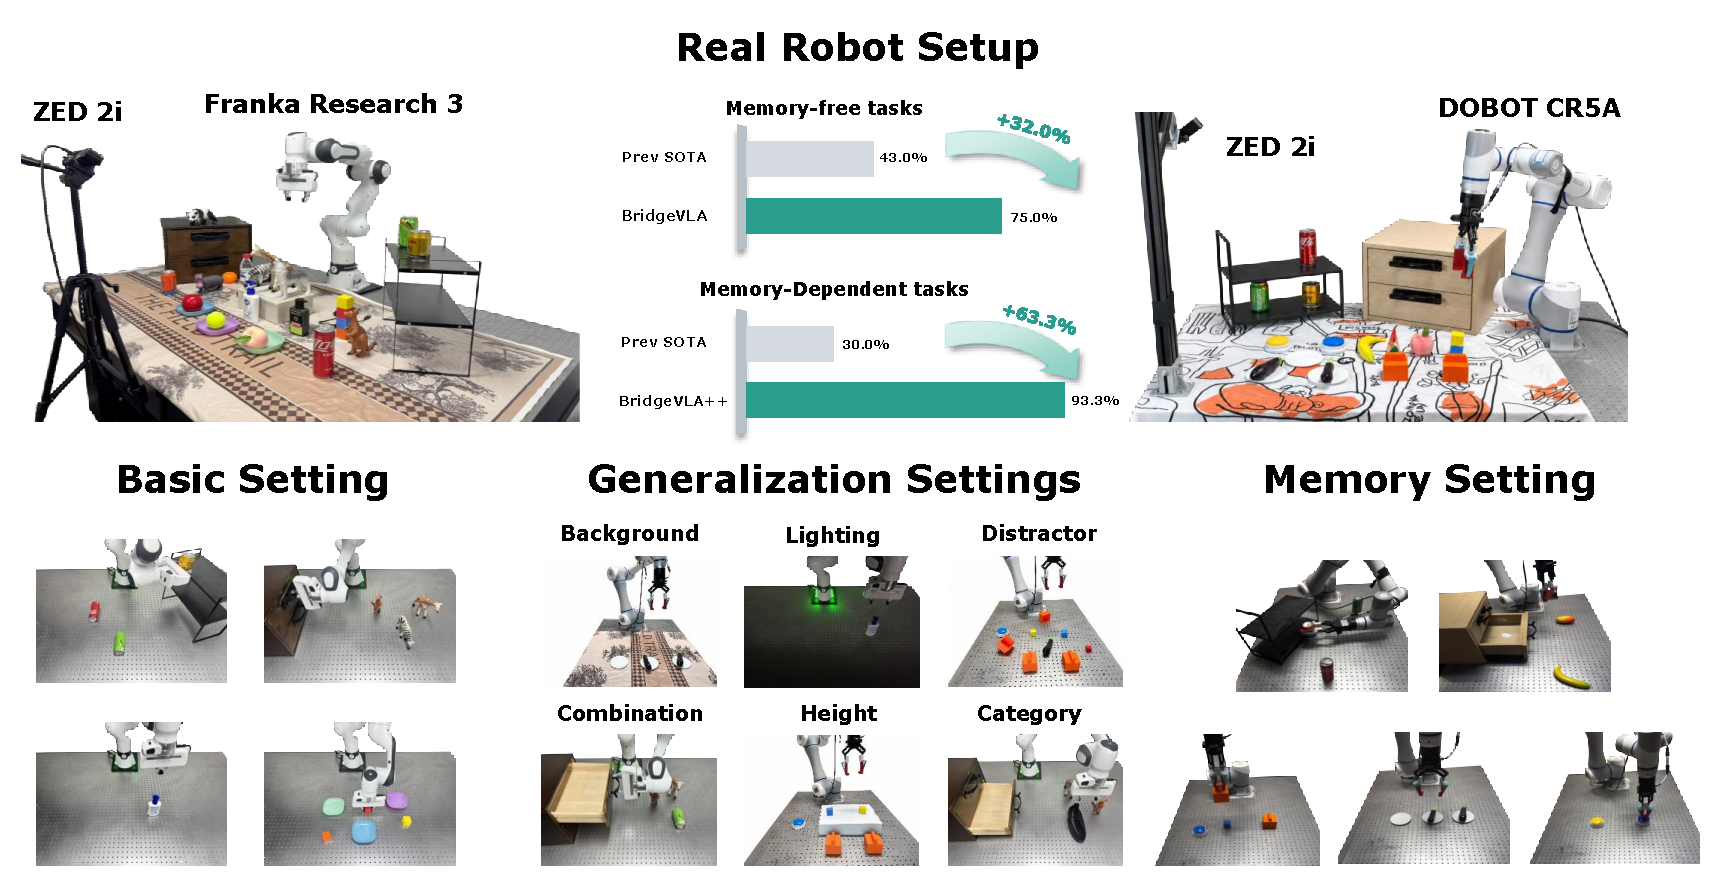
\includegraphics[width=\textwidth]{figures/real_setting_overview.pdf}
  \caption{\textbf{Real-Robot Evaluation Setup.}
  \emph{Top left:} the general-manipulation platform---a 7-DoF Franka
  Research~3 arm observed by a static ZED~2i stereo camera.
  \emph{Top right:} the memory platform---a 6-DoF Dobot CR5A arm with
  the same camera configuration.
  \emph{Bottom:} the evaluation settings of the two suites.
  The bars at the top show the average gain of our models over the
  strongest prior method in each task group: RVT-2 across the seven
  Franka settings and SAM2Act+ in the Dobot basic setting.}
  \label{fig:real_setup}
\end{figure*}

\subsubsection{General Manipulation}

\paragraph{Setup}
We evaluate \method\ on a 7-DoF Franka Research 3 manipulator with a parallel-jaw gripper, observed via a static ZED~2i depth camera (Fig.~\ref{fig:real_setup}). The evaluation covers 13 tasks ranging from simple pick-and-place to complex long-horizon manipulation, with 10 expert demonstrations per task for training. Beyond the basic setting, we design six challenging generalization settings: Distractor, Lighting, Background, Height, Combination (unseen object--skill pairings), and Category (unseen object categories). Full setup details, per-task results, and analyses are provided in Appendix~\ref{app:real_franka}.
\begin{table*}[!t]
\centering
\caption{\textbf{Real-Robot Results on Franka in the Basic Setting.}
Success counts on the 13 real-robot tasks; all evaluations are our
own, with 10 trials per task per method
(Appendix~\ref{app:eval_protocol}).
All methods are trained with 10 demonstrations per task, except
SpatialVLA~(50 demos) and the \method~(3 demos) reference row; ACT is
trained single-task, as it is not language-conditioned.
Best result per column in bold (the 3-demonstration row is excluded
from the comparison).}
\label{tab:real_robot}
\footnotesize
\setlength{\tabcolsep}{4pt}
% zero rule separation; \arraystretch below compensates the row height
\setlength{\aboverulesep}{0pt}
\setlength{\belowrulesep}{0pt}
\renewcommand{\arraystretch}{1.25}
\resizebox{\fitwidth}{!}{%
\begin{tabular}{l*{7}{c}}
\toprule
& \textbf{Avg.} & \textbf{Soda Can} & \textbf{Giraffe} & \textbf{Red Block} & \textbf{Press} & \textbf{RedBull} & \textbf{RedBull} \\
\multirow{-2}{*}{\textbf{Method}}
& \textbf{SR (\%) $\uparrow$} & \textbf{Bottom Shelf} & \textbf{Lower Drawer} & \textbf{Blue Plate} & \textbf{Sanitizer} & \textbf{Top Shelf} & \textbf{Bottom Shelf} \\
\midrule
SpatialVLA~(50)~\cite{qu2025spatialvla} & 28.5 & 1/10 & 1/10 & 5/10 & 6/10 & 3/10 & 1/10 \\
SpatialVLA~(10)~\cite{qu2025spatialvla} & 3.1  & 0/10 & 0/10 & 0/10 & 2/10 & 0/10 & 0/10 \\
$\pi_{0.5}$~\cite{intelligence2025pi_}            & 20.0 & 2/10 & 1/10 & 4/10 & 4/10 & 1/10 & 1/10 \\
ACT~\cite{zhao2023learning}             & 21.5 & 2/10 & 2/10 & 3/10 & 2/10 & 3/10 & 1/10 \\
RVT-2~\cite{goyal2024rvt}               & 90.0   & \textbf{10/10} & 8/10 & 8/10 & \textbf{10/10} & 9/10 & \textbf{10/10} \\
\midrule
\method~(3 demos) & 95.4 & 9/10 & 10/10 & 10/10 & 10/10 & 9/10 & 10/10 \\
\textbf{\method} & \textbf{96.9} & 9/10 & \textbf{9/10} & \textbf{10/10} & \textbf{10/10} & \textbf{10/10} & \textbf{10/10} \\
\bottomrule
\addlinespace[5pt]
& \textbf{Coke} & \textbf{Orange Block} & \textbf{Red Block} & \textbf{Yellow Block} & \textbf{Zebra} & \textbf{Zebra} & \textbf{Wolf} \\
\multirow{-2}{*}{\textbf{Method}}
& \textbf{Top Shelf} & \textbf{Green Plate} & \textbf{Purple Plate} & \textbf{Green Plate} & \textbf{Upper Drawer} & \textbf{Lower Drawer} & \textbf{Upper Drawer} \\
\midrule
SpatialVLA~(50)~\cite{qu2025spatialvla} & 2/10 & 6/10 & 3/10 & 5/10 & 2/10 & 0/10 & 2/10 \\
SpatialVLA~(10)~\cite{qu2025spatialvla} & 0/10 & 1/10 & 1/10 & 0/10 & 0/10 & 0/10 & 0/10 \\
$\pi_{0.5}$~\cite{intelligence2025pi_}           & 2/10 & 4/10 & 3/10 & 3/10 & 0/10 & 0/10 & 1/10 \\
ACT~\cite{zhao2023learning}             & 2/10 & 2/10 & 3/10 & 4/10 & 1/10 & 2/10 & 1/10 \\
RVT-2~\cite{goyal2024rvt}               & \textbf{10/10} & \textbf{10/10} & 9/10 & 9/10 & 7/10 & 8/10 & \textbf{9/10} \\
\midrule
\method~(3 demos) & 10/10 & 10/10 & 10/10 & 10/10 & 9/10 & 10/10 & 7/10 \\
\textbf{\method} & \textbf{10/10} & \textbf{10/10} & \textbf{10/10} & \textbf{10/10} & \textbf{9/10} & \textbf{10/10} & \textbf{9/10} \\
\bottomrule
\end{tabular}%
}
\end{table*}


\paragraph{Results}
To demonstrate the advantages of \method over existing manipulation
policies, we compare it with four representative baselines spanning different
model categories: SpatialVLA~\cite{qu2025spatialvla}, a 3D VLA model;
$\pi_{0.5}$~\cite{intelligence2025pi_}, a 2D VLA model;
ACT~\cite{zhao2023learning}, a 2D non-VLA policy; and
RVT-2~\cite{goyal2024rvt}, a 3D non-VLA policy.

We first evaluate all methods under the basic setting.
For each task, every method is evaluated over 10 trials.
To ensure a fair comparison, we photograph each test scene and manually
reproduce the same scene configuration across methods.
The results are reported in Table~\ref{tab:real_robot}.
When trained with only 10 trajectories per task, most baselines fail almost
completely, whereas the two methods that explicitly exploit 3D spatial
structure, RVT-2 and \method, achieve substantially stronger performance.
Notably, although SpatialVLA also incorporates 3D information, it remains
considerably less data-efficient.
Even when its training set is increased to 50 trajectories per task, its
success rate remains substantially lower than that of \method.
This result suggests that incorporating 3D information alone is insufficient
for constructing a data-efficient 3D VLA model; the architectural design used
to align the observation and action spaces is also critical.

Remarkably, when the training data are further reduced to only three
demonstrations per task, \method still achieves a success rate of 95.4\%,
highlighting its exceptional sample efficiency and directly addressing Q4.
Because only RVT-2 and \method achieve reliable performance under the basic
setting, we further compare these two methods across the remaining
generalization settings.
As summarized in Fig.~\ref{fig:real_results}, \method consistently
outperforms RVT-2 across all seven settings, with an average improvement of
32\%.
The gains are particularly pronounced under novel lighting conditions and
unseen object--skill combinations, demonstrating that \method can
effectively transfer the semantic knowledge of the pre-trained VLM to
real-world manipulation.
Additional details on the experimental setup, baseline implementations,
per-task results, and analyses are provided in
Appendix~\ref{app:real_franka}.
\begin{figure}[t]
  \centering
  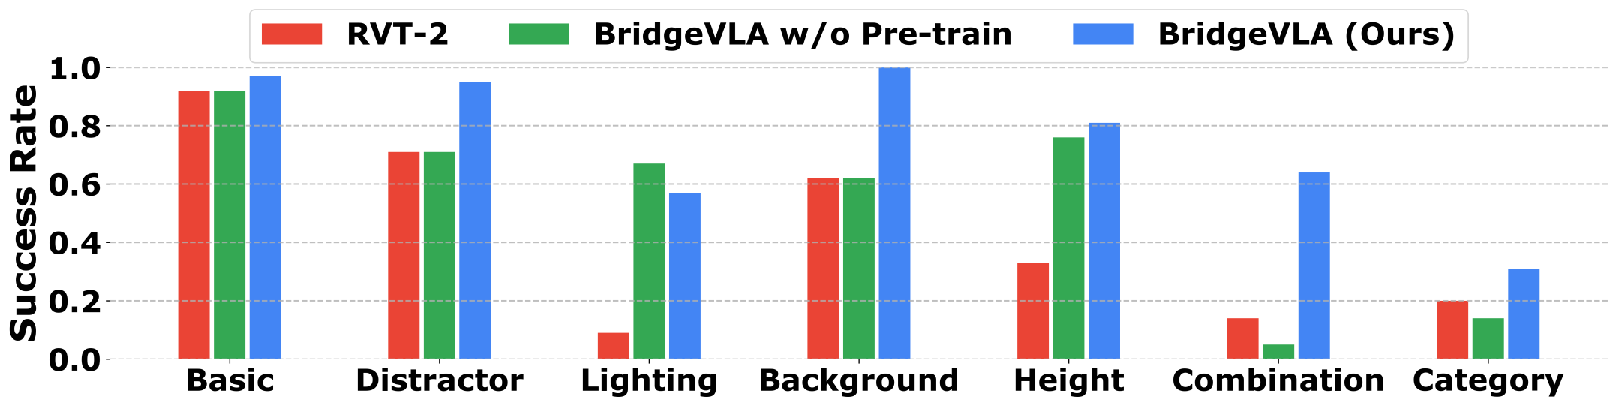
\includegraphics[width=\columnwidth]{figures/BridgeVLA_real_results.pdf}
  \caption{\textbf{Real-Robot Generalization Results.}
  Average success rate over the 13 Franka tasks in the basic setting and
  the six generalization settings;
  the \emph{w/o Pre-train} bars ablate the 2D-heatmap pre-training
  (Sec.~\ref{sec:exp:ablation}).}
  \label{fig:real_results}
\end{figure}

\subsubsection{Memory-Augmented Manipulation}
\paragraph{Setup}
To validate \memmethod\ in the real world, we deploy the model on a Dobot CR5A equipped with an external RGB-D camera to capture the workspace (Fig.~\ref{fig:real_setup}). The evaluation suite pairs three memory-dependent tasks---\emph{Cover Blocks}, \emph{Press Button}, and \emph{Swap Eggplant}---with two memory-free standard manipulation tasks, \emph{Put in Drawer} and \emph{Put on Shelf}. The former probe whether the spatio-temporal memory transfers to physical hardware; the latter verify that the memory extension does not erode the policy's general manipulation capability. Each memory-dependent task is driven by a single language instruction, while \emph{Put in Drawer} and \emph{Put on Shelf} use two instructions that differ in target height. Similar to the setup on the Franka platform, we train on 10 demonstrations per language instruction and evaluate every instruction over 10 trials in each of five settings---Basic, Distractor, Background, Height, and Lighting---against memory-free \method\ and the memory-augmented SAM2Act+~\cite{fang2025sam2act}. Full details are provided in Appendix~\ref{app:real_dobot}.

\paragraph{Results}
Consistent with our simulation findings, the proposed spatio-temporal memory effectively transfers to physical hardware. In the basic setting (Table~\ref{tab:real_dobot_basic}), \memmethod\ achieves an average success rate of 93.3\% on the three memory-dependent tasks, yielding a threefold improvement over the memory-augmented SAM2Act+ (30.0\%). Conversely, the memory-free \method\ largely fails (20.0\%), confirming that these tasks intrinsically require episodic memory. This substantial performance margin over SAM2Act+ stems from architectural differences in memory management. Because SAM2Act+ indiscriminately stores every step and retrieves only a fixed temporal window, near-duplicate frames tend to dilute critical historical information. \memmethod\ overcomes this limitation via its targeted spatio-temporal memory design (Sec.~\ref{sec:memmethod}). Furthermore, owing to its pre-trained VLM backbone, \memmethod\ exhibits strong robustness against visual disturbances (Table~\ref{tab:real_dobot_generalization}). Importantly, this memory integration comes at no cost to general manipulation capabilities: on the two memory-free tasks, \memmethod\ matches or exceeds \method\ in both success rate and generalization across all settings. Collectively, these results demonstrate that \memmethod\ successfully acquires memory-dependent competencies in real-world scenarios while fully preserving the foundational manipulation skills and visual robustness of the base model. Per-instruction counts are detailed in Table~\ref{tab:app:real_dobot_all}.
\begin{table}[!t]
\centering
\caption{\textbf{Per-task success rates on the real Dobot platform in the
basic setting.}
Ten trials per language instruction; \emph{Mem.}\ marks memory-augmented
policies.
\emph{Put in Drawer} and \emph{Put on Shelf} are each evaluated with two
instructions (upper and lower target) and are reported as their average;
per-instruction counts are given in Table~\ref{tab:app:real_dobot_all}.}
\label{tab:real_dobot_basic}
\footnotesize
\setlength{\tabcolsep}{3pt}
% zero rule separation; \arraystretch below compensates the row height
\setlength{\aboverulesep}{0pt}
\setlength{\belowrulesep}{0pt}
\renewcommand{\arraystretch}{1.25}
\begin{tabular}{lcccccc}
\toprule
& & \multicolumn{3}{c}{\textbf{Memory-Dependent}}
& \multicolumn{2}{c}{\textbf{Memory-Free}} \\
\cmidrule(lr){3-5}\cmidrule(lr){6-7}
\textbf{Method}
& \textbf{Mem.}
& \textbf{\makecell{Cover\\Blocks}}
& \textbf{\makecell{Press\\Button}}
& \textbf{\makecell{Swap\\Eggplant}}
& \textbf{\makecell{Put in\\Drawer}}
& \textbf{\makecell{Put on\\Shelf}} \\
\midrule
SAM2Act+~\cite{fang2025sam2act} & \cmark & 20.0\% & 0.0\% & 70.0\% & 60.0\% & 20.0\% \\
\textbf{\method} & \xmark & 0.0\% & 0.0\% & 60.0\% & 100.0\% & 90.0\% \\
\textbf{\memmethod} & \cmark & 100.0\% & 100.0\% & 80.0\% & 100.0\% & 100.0\% \\
\bottomrule
\end{tabular}
\end{table}

\begin{table}[!t]
\centering
\caption{\textbf{Success rates on the real Dobot platform across all
evaluation settings.}
Each entry is the mean over the three memory-dependent or two
memory-free tasks of Table~\ref{tab:real_dobot_basic}; \emph{Avg.}\
averages the four disturbance settings.
\emph{Mem.}\ marks memory-augmented policies; per-instruction counts
are given in Table~\ref{tab:app:real_dobot_all}.}
\label{tab:real_dobot_generalization}
\footnotesize
\setlength{\tabcolsep}{3pt}
% zero rule separation; \arraystretch below compensates the row height
\setlength{\aboverulesep}{0pt}
\setlength{\belowrulesep}{0pt}
\renewcommand{\arraystretch}{1.25}
\resizebox{\fitwidth}{!}{%
\begin{tabular}{lccccccc}
\toprule
& & & \multicolumn{5}{c}{\textbf{Visual Disturbance}} \\
\cmidrule(lr){4-8}
\textbf{Method}
& \textbf{Mem.}
& \textbf{Basic}
& \textbf{Distractor}
& \textbf{Background}
& \textbf{Height}
& \textbf{Lighting}
& \textbf{Avg.} \\
\midrule
\multicolumn{8}{@{}l}{\emph{Memory-dependent tasks}} \\
SAM2Act+~\cite{fang2025sam2act} & \cmark & 30.0\% & 0.0\% & 0.0\% & 0.0\% & 3.3\% & 0.8\% \\
\textbf{\method} & \xmark & 20.0\% & 20.0\% & 23.3\% & 6.7\% & 13.3\% & 15.8\% \\
\textbf{\memmethod} & \cmark & 93.3\% & 73.3\% & 86.7\% & 76.7\% & 76.7\% & 78.3\% \\
\midrule
\multicolumn{8}{@{}l}{\emph{Memory-free tasks}} \\
SAM2Act+~\cite{fang2025sam2act} & \cmark & 40.0\% & 0.0\% & 0.0\% & 0.0\% & 7.5\% & 1.9\% \\
\textbf{\method} & \xmark & 95.0\% & 57.5\% & 72.5\% & 67.5\% & 67.5\% & 66.3\% \\
\textbf{\memmethod} & \cmark & 100.0\% & 70.0\% & 100.0\% & 82.5\% & 75.0\% & 81.9\% \\
\bottomrule
\end{tabular}}
\end{table}


\subsection{Ablation Studies}
\label{sec:exp:ablation}

To address Q3, we conduct two groups of ablation studies: we first ablate the core architectural designs of the base model \method\ (upper ablation rows of Table~\ref{tab:rlbench}), and then dissect the spatio-temporal memory of \memmethod\ (lower ablation rows of Table~\ref{tab:rlbench} and Table~\ref{tab:rmbench_ablation}).

\textbf{Whether we need to predict heatmaps before predicting actions.}
Replacing the convex upsampling module with a parameter-matched Transformer decoder that directly regresses target positions (Appendix~\ref{app:finetune_hparams}) causes the average success rate on RLBench to collapse from 90.5\% to 31.4\% (Table~\ref{tab:rlbench}).
The ablated model is also markedly harder to optimize, demanding a threefold larger batch size (192 vs. 64) and careful learning-rate tuning.
We attribute this gap to three properties of the heatmap as an intermediate representation: it provides denser supervision than sparse 3D position vectors, the 3D-to-2D projection injects a helpful spatial prior, and the heatmaps share the spatial structure of the input images, keeping input and output aligned.

\textbf{Whether we need to remove the 3D position input to the VLM backbone.}
Unlike typical 3D VLA models such as SpatialVLA, \method\ feeds the backbone only RGB projection images.
Fusing per-pixel 3D positions into the image features via a 3D convolutional module (Appendix~\ref{app:finetune_hparams}) injects richer spatial cues, yet degrades the success rate from 90.5\% to 56.2\% (Table~\ref{tab:rlbench}), which we attribute to the resulting shift of the image features away from the distribution seen during VLM pre-training.
For a pre-trained VLM, preserving input alignment thus outweighs adding explicit 3D inputs.

\textbf{Whether we need the 2D heatmap pre-training.}
Without the pre-training stage, \method\ w/o Pre-train fails to generalize in both language-related real-world settings and cannot even match RVT-2, whereas the full \method\ performs best in both, especially in Combination (Fig.~\ref{fig:real_results}).
We hypothesize that the 2D heatmap pre-training teaches the model to ground language semantics in image observations directly within the heatmap space, an ability that fine-tuning on a handful of robot trajectories alone cannot instill.

\textbf{Whether a continuous rotation representation outperforms a discretized one.}
Replacing the continuous 6D rotation representation (Sec.~\ref{sec:bridgevla:finetune}) with the discretized per-axis Euler-angle classification head from our preliminary conference version degrades the RLBench average from 90.5\% to 88.2\% (Table~\ref{tab:rlbench}), with the drop concentrated in tasks demanding high-precision end-effector orientations.
The 6D representation also stays robust in near-vertical gripper poses, avoiding the gimbal lock inherent to discretized Euler angles (Appendix~\ref{app:finetune_hparams}).

\textbf{Whether we need the spatial memory $\mathcal{S}$.}
Since $\mathcal{S}$ targets fine-grained geometric alignment under arm-induced occlusions (Sec.~\ref{sec:memmethod:spatial}), we ablate it mainly on RLBench, whose precision tasks are exactly where such occlusions arise.
Removing $\mathcal{S}$ lowers the RLBench average of \memmethod\ (93.7\% vs. 92.0\%), and the loss concentrates exactly in occlusion-heavy precision tasks, \eg, \emph{Sort Shape} (72.0\% vs. 60.8\%, Table~\ref{tab:rlbench}); on RMBench, whose tasks stress temporal sequencing rather than geometric alignment, the removal is nearly harmless (Table~\ref{tab:rmbench_ablation}).
This benchmark-selective effect indicates that $\mathcal{S}$ contributes complementary geometric detail for precise alignment rather than duplicating the temporal memory.

\textbf{Whether we need the temporal memory $\mathcal{T}$.}
Removing $\mathcal{T}$ collapses the RMBench success rate of \memmethod\ from 96.0\% to 21.3\%, close to the memory-free base model (18.9\%, Table~\ref{tab:rmbench_ablation}).
Notably, $\mathcal{T}$ also benefits RLBench (93.7\% vs. 91.9\%) despite its tasks not being intrinsically memory-dependent: the anchor views and neighboring keyframes provide a stable global reference and local motion cues that help general manipulation (Table~\ref{tab:rlbench}).

All the above results address Q3: heatmap-based action prediction, input alignment, and the temporal memory account for the largest gains; the heatmap pre-training underpins language-conditioned generalization; and the continuous rotation and the spatial memory contribute smaller, targeted gains on orientation-critical and occlusion-heavy tasks, respectively.
